\documentclass[final, 11pt]{article}

\usepackage[italian]{babel}
\usepackage{braket}
\usepackage{diagbox} 
%\usepackage{setspace}
\usepackage{tikz}

\usepackage{amsmath}
\usepackage{amsfonts}
\usepackage{algorithm}		%pseudocodice package
\usepackage{algorithmic}	%pseudocodice package

\usepackage[utf8]{inputenc}

\usepackage{listings}
\usepackage{xcolor}


\usepackage{graphicx}
\usepackage{pdfpages}
\title{Studio di framework per la generazione di fake images di vestiti: Analisi e confronto dei codici VITON e Virtual Try-On with Detail Carving}
\author{ Candidato: Fabio Tarocco VR421748}
\begin{document}
	\clearpage
	
\begin{titlepage}
	\centering
	\vspace*{\fill}
	{\scshape\LARGE Università degli Studi di Verona \par}
	\vspace{1.5cm}
	{\huge Studio di framework per la generazione di fake images di vestiti: Analisi e confronto dei codici VITON e Virtual Try-On with Detail Carving \par}
	\vspace{0.5cm}
	{\scshape  Corso di Laurea Triennale in Informatica \par}
	\vspace{1cm}
	{\Large\itshape Fabio Tarocco VR421748 \par}
	\vspace{1cm}
	\vspace{5cm}
	\vspace*{\fill}
	{\large 16 Ottobre 2020 \par}
\end{titlepage}
	\newpage
	\thispagestyle{plain} % empty
	\mbox{}
	\clearpage
	
	\tableofcontents
	\newpage
	\section{Introduzione al report}
	\subsection{Idea di base}
	La proposta iniziale di stage era quella di analizzare alcuni framework per il riconoscimento dai FAKE images attraverso l’utilizzo di NN e Deep Learning. L’idea era alquanto interessante.
	Per procedere con l’esperienza si è deciso di andare a capire il funzionamento di quello che c’è a monte delle FAKE-IMAGES, cioè la loro creazione.
	
	Si è passati quindi ad un progetto che andasse a studiare il funzionamento e la qualità dei risultati di Frame Work per i virtual Try-On (VTO). La generazione, quindi, di immagini false, artefatte, create attraverso l’utilizzo di codice basato su Reti neurali e Machine Learning, ad hoc per l’ambito della moda e non solo.\\
	Il punto di partenza è stato il codice VITON (portato al CVPR 2018). Una rete per il try-on virtuale image-based (partendo da un dataset di immagini 2D con l’obbiettivo di creare modelli 3D). Codice che sarà la base di partenza e di confronto con gli altri analizzati durante l’esperienza.
	Proseguendo poi al ricercare un concorrente, sempre basato su VITON, per permettere dei confronti prestazionali, nel caso analizzato è stato utilizzato Virtual Try-on with Detail Carving (VTODC). Framework portato al CVPR 2019 e realizzato dalla JDAI CV, con sede a Pechino, che introduce la possibilità di scegliere anche con quale posa generare il modello finale, oltre all’abito e al soggetto.
	
	Infine si è deciso di produrre una demo che permettesse di scegliere una combinazione di soggetti/abiti da un dataset limitato ed eseguire la sostituzione del vestiario con l’opzione di poter introdurre modifiche riguardanti la suddivisione fra i vari segmenti che compongono soggetto di base: vestito, braccia/maniche, pantaloni, viso e capelli.
	
	\subsection {Obiettivi tirocinio}
	L'obbiettivo che ci si è posti come cardine dell'esperienza di tirocinio è stato quello di valutare i risultati, quindi le prestazioni, di più codici che eseguono virtual try-on con base (VITON).
	
	Le richieste erano quelle di capire quando i due codici confrontati producevano output validi e quando invece presentavano difficoltà nel produrli.
	Si è quindi proceduto ad analizzare diversi codici basati sul predecessore VITON e scegliere quelli che potevano avere incrementi sostanziali e visibili nelle prestazioni e nella qualità/affidabilità dei risultati.
	
	Durante l'esperienza si è inoltre deciso di provare ad aggiungere ulteriori obiettivi ossia: Produrre un piccolo applicativo "CANVAS" che permettesse la modifica del label (suddivisione delle componenti del soggetto finale: viso, vestito, braccia, pantaloni, capelli) e applicarlo poi ad una demo "PITON" che permettesse ad un utente di generare differenti outfit, attraverso l'utilizzo di un dataset di campioni ridotto, potendo inoltre utilizzare CANVAS per modificare alcune caratteristiche degli abiti/soggetto.
	
	
	
	\subsection{Cos'è un Virtual Try-On}
	Partiamo spiegando cos'è un virtual try-on. 
	
	È una modalità alternativa con la quale un futuro cliente di un negozio di abbigliamento o di gioielli potrà provare i prodotti dei negozi in modo virtuale, senza dover fisicamente provarli in camerino. Quindi attraverso l'utilizzo di un dispositivo dotato di fotocamera, l'utente può valutare se comprare o meno un capo provandolo virtualmente, attraverso l'utilizzo di realtà aumentata.
	
	Questo approccio, già presente da anni sul mercato ma migliorato mediante l'utilizzo di machine learning
e modelling 3D, permette di provare un capo prima di acquistarlo in qualsiasi luogo, senza l'"obbligo" di andare in negozio, di provare contemporaneamente più capi, valutando anche i vari outfit e soprattutto è time-saving.
	
	Nel caso preso in esame si è operato su codici che prevedevano l'utilizzo di dataset di immagini prese da
un catalogo di abbigliamento di un negozio di e-commerce, quindi non attraverso l'utilizzo di modelling 3D e risultati real-time applicati su video, ma sulla creazione di outfit alternativi a quelli originali utilizzando le coppie modello target e vestito target.
	
	\begin{figure}[!htb]
		\begin{center}
			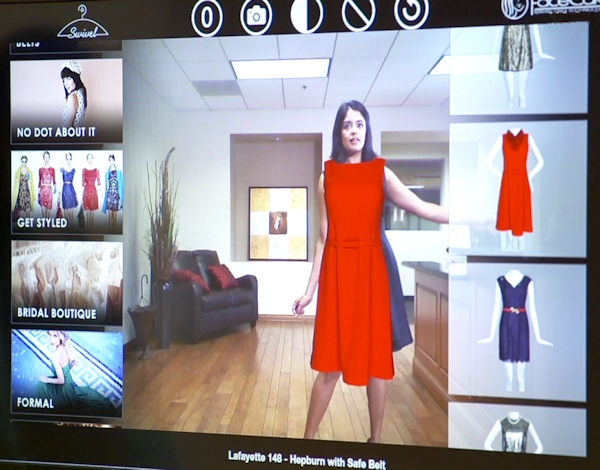
\includegraphics[scale=.7]{FaceCake-virtual-dressing-room.jpg}
		\end{center} \caption{Dressing room dotata di VTO in real time}
	\end{figure} 

	\section{VITON}
	\subsection{Descrizione codice}
	dsad
	\subsection{Qualità output prodotti}
	
	\newpage
	\section{VTO con Detail Carving}
	dsads
	\subsection{Descrizione codice}	
	dsa
	\subsection{Qualità output prodotti}
	Si valutano i segnali che vengono proposti nell'esercizio. Il primo è definito come un segnale con supporto illimitato e con frequenza massima 
	
	\newpage
	\section{Confronto risultati fra i due framework}	
	Si valutano i segnali che vengono proposti nell'esercizio. Il primo è definito come un segnale con supporto illimitato e con frequenza massima 
	
	\newpage
	\section{Demo PyTryOn: applicazione di ACGPN}
	\subsection{Introduzione alla Demo}
	L’applicativo che si è deciso di produrre doveva soddisfare due requisiti principali:
	\begin{itemize}
		\item Permettere all’utente la possibilità di scegliere la coppia Modello-Abito
		\item Modifica delle segmentazioni relative alle componenti che formavano l’immagine di base:
		Ciano= capelli, Violetto = viso, Azzurro = Abito, Giallo = Pantaloni, Arancio/Rosso = Braccio DX
		Verde = Braccio SX
	\end{itemize}

	\begin{figure}[!htb]
		\begin{center}
			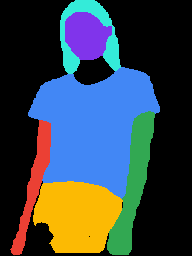
\includegraphics[scale=.7]{002474_0.png}
		\end{center} \caption{Schema colore della suddivione addottata nei Label da ACGPN}
	\end{figure} 
	
	È stato scelto come Framework per la sostituzione dell’abito il sorgente ACGPN, portato all’CVPR nell’edizione 2020. 
	Sistema realizzato nell’ambiente di sviluppo CUDA ossia l'architettura hardware creata da NVIDIA per consentire l’elaborazione parallela. Per eseguire questo codice è stato necessario l’utilizzo di macchine più performanti ed è stato possibile grazie all’accesso alle macchine dell’Università di Verona, su cui si è lavorato tramite SSH.
	
	
	PyTryOn è formato da due componenti principali: la prima è il wrapper che contiene CANVAS (app per la modifica dei label) e lo script per la selezione delle immagini sorgenti dal dataset di cui è dotato il programma, la seconda invece, è l’eseguibile test.py contenuto nella sezione di ACGPN dedicata alle fasi di testing, ossia quella di Inference.
	
	Tralasciando le parti già presenti nella repository iniziale di ACGPN, il codice è stato scritto completamente in Python. Il codice di PyTryOn è poi stato portato all’interno dell’ambiente di lavoro di ACPGN in modo da aver accesso diretto a test.py e soprattutto al Dataset.
	
	Per quanto riguarda quest’ultima componente, il dataset utilizzato nella demo prodotta è un sottoinsieme di quello utilizzato per ACGPN e VITON. Per le fasi di test e debugging si è optato per un dataset della dimensione di 5 modelli e 5 abiti scelti in modo casuale da quello originale, selezionando quelle immagini che non portassero a problemi di Missing keypoints o deformazioni varie nel risultato (stessi problemi riscontrati nei test di VITON).
	
	\subsection{Descrizione interfaccia}
	Quello che l’utente si trova davanti è un’interfaccia minimale e alquanto spartana, non era necessario aggiungere tanti dettagli, ma rendere il più possibile leggero l’applicativo dovendolo eseguire via SSH.
	L’interfaccia è così suddivisa:
\newline
	(1) Anteprima dei Soggetti utilizzabili come base per il VTO.
\\
	(2) Relative codifiche delle immagini dei soggetti.
\\
	(3) Menu a tendina per la selezione del soggetto. 
\\
	(4) Tasto avviare l’applicativo per la modifica delle suddivisioni del soggetto. 
\\
	(5) Anteprima degli Abiti utilizzabili come target per il VTO. 
\\
	(6) Come sopra, relative codifiche delle immagini degli abiti. \\
	(7) Menu a tendina per la selezione degli abiti.
\\
	(8) Avvio del file di test.py per la produzione del risultato. 
\\
	
	
	
	Passando all’interfaccia della mini applicazione per la modifica delle segmentazioni “CANVAS” abbiamo:
\newline
	(9) Menù a tendina per la selezione di import/export dell’immagine da modificare. \\
	(10) Menu a tendina per la selezione del colore del pennello in base alla parte della segmentazione che si vuole modificare. 
\\
	(11) Cursore per la selezione della dimensione del pennello. 
\\
	(12) Tasto reset, per rimuovere l’immagine che si stava modificando. \\
	(13) Piano di disegno su cui si può modificare l’immagine sorgente.
\\
	
	\subsection{Funzionamento}
	La componente principale che ci permette di modificare le segmentazioni in cui il modello è suddiviso in modo chiaro e intuitivo è resa possibile grazie all’utilizzo di uno script di conversione da Grey Scale a RGB seguendo gli assegnamenti che sono stati scelti dagli sviluppatori di ACGPN. 
	
	Nel momento in cui si va a selezionare una delle immagini che si vuole modificare, viene effettuata la conversione e aperta sulla tavola, viceversa, quando si va ad effettuare il salvataggio si passa da RGB a GreyScale. Per effettuare questa conversione abbiamo utilizzato un due cicli annidati e tenendo conto delle varie codifica/valori che ogni pixel assumeva, si andava a sostituire con il codice coloro corrispondente alla controparte convertita.
	
	Questo applicativo è stato creato utilizzando i pacchetti TKINTER e PILLOW, il primo per generare GUI su Python mentre il secondo utilizzato ogniqualvolta si devono manipolare immagini, aprirle o salvarle.
	Utilizzando questi pacchetti è stata generata anche l’interfaccia e il codice dell’applicativo principale “DEMO\_pyvton”, ossia quello che racchiude CAVAS e il test.py per il lancio del VTO.
	
	In questa parte non c’è nulla di articolato, viene data la possibilità all’utente di scegliere l’outfit e il soggetto mediante l’utilizzo di due menu a tendina con i relativi codici dei campioni proposti ed inoltre è presente il tasto per l’avvio di CANVAS.
	
	L’altro tasto presente nell’interfaccia principale (4) è quello per l’avvio del virtual try-on, quindi dello script per il testing di ACGPN.
	Il sistema di ACGPN utilizza input diversi rispetto alle due alternative proposte in precedenza: VITON e VTODC, infatti richiede:
	\begin{itemize}
		\item Abito target
		\item Modello di base
		\item Label del modello in grayscale
		\item Edge degli abiti
		\item Keypoints del soggetto in formato json
	\end{itemize}
	Durante l’utilizzo dell’applicativo è possibile modificare 3 dei 5 punti utilizzati come input, ossia i primi 3.
	
	\subsection{Risultati}
	Quello che è stato ottenuto dai vari testing della demo è un risultato non molto eclatante, infatti, ACGPN sembra ignorare in gran parte le modifiche che vengono applicate sul label di input, il quale viene sostituito, in fase di ricostruzione del risultato finale, con uno generato dal codice.
	Il label che si va a modificare viene preso in considerazione in modo marginale, viene anzi, effettuate delle modifiche ulteriori su di esso per migliorare la resa dell’abito target sul soggetto target, tendendo conto delle condizioni iniziali e finali a cui si vuole arrivare. 
	Queste possono essere suddivise in 3 alternative:
	\begin{enumerate}
		\item Il soggetto iniziale presenta un abito a maniche lunghe mentre l’abito target è a maniche corte, comporta la mancanza di riferimenti per la ricostruzione delle braccia scoperte e per risolvere questo interviene ACGPN
		\item Il soggetto target presente un abito a maniche corte mentre l’abito d’arrivo è a maniche lunghe, semplicemente avviene una sovrapposizione, seguendo il wrapping corretto, dell’abito sul soggetto
		\item Il vestito target è più corto di quello del soggetto target. In questo caso il risultato che si ottiene e simile a quelli ottenuti con VITON, quindi una fusione fra abito e pantalone a chiazze.
	\end{enumerate}
	
	
\end{document}